	\documentclass[
	12pt,
	]{article}
	\usepackage{subcaption}
	\usepackage{changepage}
	\usepackage{titlesec}
	\usepackage{graphicx}
	\usepackage{graphics}
	\usepackage{booktabs}
	\usepackage{amsmath}
	\usepackage{siunitx}
	\usepackage{physics}
	\usepackage{amssymb}
	\usepackage{mathrsfs}
	\usepackage{undertilde}
	\usepackage{dutchcal}
	\usepackage{amsthm}
	\usepackage{wrapfig}
	\newcommand{\tx}{\text{}}
	\usepackage{tikz}
	\usepackage{xfrac}
	\newcommand{\td}{\text{dim}}
	\newcommand{\tvw}{T : V\xrightarrow{} W }
	\newcommand{\ttt}{\widetilde{T}}
	\newcommand{\ex}{\textbf{Example}}
	\newcommand{\aR}{\alpha \in \mathbb{R}}
	\newcommand{\abR}{\alpha \beta \in \mathbb{R}}
	\newcommand{\un}{u_1 , u_2 , \dots , n}
	\newcommand{\an}{\alpha_1, \alpha_2, \dots, \alpha_2 }
	\newcommand{\sS}{\text{Span}(\mathcal{S})}
	\newcommand{\sSt}{($\mathcal{S}$)}
	\newcommand{\la}{\langle}
	\newcommand{\ra}{\rangle}
	
	\usepackage{mathtools}
	\DeclarePairedDelimiter{\norm}{\lVert}{\rVert}
	\newcommand{\vectorproj}[2][]{\textit{proj}_{\vect{#1}}\vect{#2}}
	\newcommand{\vect}{\mathbf}
	\newcommand{\uuuu}{\sum_{i=1}^{n}\frac{<u,u_i}{<u_i,u_i>} u_i}
	\newcommand{\B}{\mathcal{B}}
	\newcommand{\Ss}{\mathcal{S}}
	
	\newtheorem{theorem}{Theorem}[section]
	\theoremstyle{definition}
	\newtheorem{corollary}{Corollary}[theorem]
	\theoremstyle{definition}
	\newtheorem{lemma}[theorem]{Lemma}
	\theoremstyle{definition}
	\newtheorem{definition}{Definition}[section]
	\theoremstyle{definition}
	\newtheorem{Proposition}{Proposition}[section]
	\theoremstyle{definition}
	\newtheorem*{example}{Example}
	\theoremstyle{example}
	\newtheorem*{note}{Note}
	\theoremstyle{note}
	\newtheorem*{remark}{Remark}
	\theoremstyle{remark}
	\newtheorem*{example2}{External Example}
	\theoremstyle{example}
	
	\title{PHYS 241 Assignment 1}
	\titleformat*{\section}{\LARGE\normalfont\fontsize{12}{12}\bfseries}
	\titleformat*{\subsection}{\Large\normalfont\fontsize{10}{15}\bfseries}
	\author{Mihail Anghelici 260928404}
	\date{\empty}
	
	\begin{document}
	\maketitle
	\section{Question 1}
		First, since the stove operates at $450 \si{\degreeCelsius}$ let us transform the temeprature coefficient of resistance.
		\begin{align*}
			 \Delta \rho &= \alpha \Delta T \rho_{0}\\
			 &= (3.5 \cross 10^{-3} \si{\per\degreeCelsius})(450 \si\degreeCelsius - 20\si\degreeCelsius)(3.2\cross 10^{-8} \si{\ohm\meter})	\\
			 &= 4.8 \cross 10^{-8} \si{\ohm\meter} 
		\end{align*}
		$$  \implies \rho = 8.0 \cross 10^{-8} \ \si{\ohm \meter}\quad \text{at $450 \si{\degreeCelsius}$} $$
		Power dessipation in a resistor is given by the following relationship
		$$ P = i^{2}R =\frac{V^{2}}{R}$$
		Therefore we can compute the resistor's resistance : 
		$$ R = \frac{V^{2}}{P} = \frac{(220)^{2}}{1000} \left[\frac{\si{\volt\squared}}{\si{\watt}}\right] = 48.4 \ \si{\ohm}$$
		from the relationship between a wire's shape and it's resistance, we can find the legnth of the wire required.
		\begin{equation*}
			 R = \rho \frac{L}{A} \implies L = \frac{RA }{\rho} =\frac{\pi d^{2} \ 48.4 \ \si{\ohm}}{4(8.0\cross 10^{-8})} \bigg[\frac{\si{\meter\squared \volt\squared}}{\si{\ohm\meter}}\bigg] = \boxed{= 29.6 \ \si{\meter}}
		\end{equation*}
		 \section{Question 2}
		 	\subsection{a) }
		 		The resistors are presented in series, therefore 
		 		$$ V_{s} = I_{s}(R_{1}+R_{2}) \implies I_{s} = \frac{V_{s}}{R_{1}+R_{2}} = \frac{5 \ \si{\volt}}{300 \ \si{\ohm}} = 16.7 \ \si{\milli\ampere}$$
		 	\subsection{b} 
		 		For resistors in series, the voltage dropped across them is directly proportional to their size ,i.e, their resistance. Thus, 
		 		$$ \Delta V_{2} = I_{s}R_{2} = \frac{1}{60} \ \si{\ampere} \ (200) \ \si{\ohm} = \frac{10}{3} \ \si{\volt} = 3.33 \ \si{\volt}$$
		 	\subsection{c) }
		 		The power dissipated in $R_{2}$ is given by the following equation : 
		 		 $$ P_{2} = i^{2} R_{2} = \left(\frac{1}{60}\right)^{2} \si{\ampere\squared} \ 200 \ \si{\ohm} =  \frac{1}{18} \ \si{\watt} = \frac{1}{18} \cross 10^{-3} \ \si{\watt} = 55.6 \ \si{\milli\watt} $$
		 \section{Question 3}
		 	The upward portion of the given circuit acts as if it had a very small resistance, let us denote it $R^{\prime}$. Since $R^{\prime}$ and $R_{1}$ are parallel,
		 	\begin{gather*}
		 		R_{T} = \left(\frac{1}{R^{\prime}} + \frac{1}{R_{1}}\right)^{-1}\\
		 	    R_{1} >> R^{\prime} \implies \frac{1}{R^{\prime}} \to \infty \implies R_{T} = \frac{1}{\infty}	
		 	\end{gather*} 
		 	Effectively, $R_{1}$ acts as if it were absent due to the given configuration.\\
		 	\subsection{a) }
		 		Consequently we can compute the current in the circuit :  
		 			$$ i = \frac{V_{0}}{R_{2}} = \frac{5 \ \si{\volt}}{200 \ \si{\ohm}} = 25 \ \si{\milli\ampere}$$
		 	\subsection{b) }
		 		\begin{align*}
		 			I  = \frac{V}{R_{2}} \implies V &= R_{2}I \\
		 			&= 200 \ \si{\ohm} \ 0.025 \ \si{\ampere} \\
		 			&=  5 \ \si{\volt}
		 		\end{align*} 
		 	\subsection{c) }
		 		The power dissipated in $R_{2}$ is given by the following equation : 
		 		\begin{align*}
		 			 P_{2} &= i^{2} R_{2}\\
		 			 &= (0.025 \ \si{\ampere})^{2} \ 200 \ \si{\ohm}  \\
		 			 &= 0.125 \ \si{\watt} = 125 \ \si{\milli\watt}
		 		\end{align*}
		 \section{Question 4}
		 	The current $I$ pasing through the right-ward portion of the parallel circuit is given by the following equation : 
		 	$$ I_{2} = \frac{V}{R_{2}} = \frac{5 \ \si{\volt}}{300 \ \si{\ohm}} = \frac{1}{60} \ \si{\ampere} = 16.7 \ \si{\milli\ampere}$$
		 \section{Question 5}
		 \begin{figure}[htp]
		 	\centering
		 	\begin{subfigure}[h]{0.3\textwidth}
		 		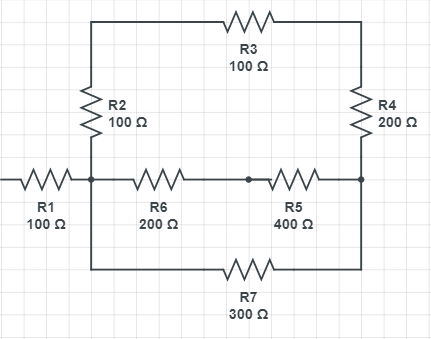
\includegraphics[width=\textwidth]{phys241_ass1_f1.png}
		 		\caption{}
		 	\end{subfigure}
		 	\hfill
		 	\begin{subfigure}[h]{0.3\textwidth}
		 		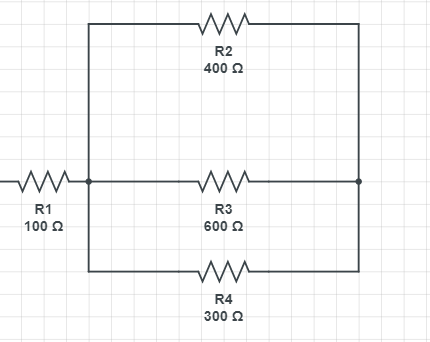
\includegraphics[width=\textwidth]{phys241_ass1_f2.png}
		 		\caption{}
		 	\end{subfigure}
		 	\hfill
		 	\begin{subfigure}[h]{0.3\textwidth}
		 		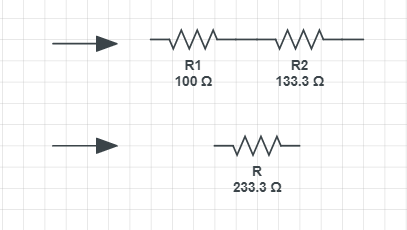
\includegraphics[width=\textwidth]{phys241_ass1_f3.png}
		 		\caption{}
		 	\end{subfigure}
		 \end{figure}
	Figure a) : Original circuit schematic.\\
		 Figure b) : $R_{2}$ , $R_{3}$ and $R_{4}$ are resistors in series, therefore they recombine to form a single resistor. Define $R_{2} = 400 \ \si{\ohm}$ the sum of the series resistors. \\
		 Figure c) :  $R_{2} , R_{3}$ and $R_{4}$ from figure $b$) are resistors in parallel therefore they recombine as $R_{2} = \sfrac{400}{3} \ \si{\ohm}$. Finally, $R_{1}$ and the recombined $R_{2}$ are in series thus the final equivalent resistor is $R= \sfrac{700}{3} \ \si{\ohm}$.
		  $$ R = \left(\frac{1}{R_{2}} + \frac{1}{R_{3}} + \frac{1}{R_{4}}\right)^{-1} = \frac{700}{3} \ \si{\ohm} = 233. 3 \ \si{\ohm}$$
		  \section{Question 6.}
		  Since there's a circuit ground inserted at point B in the middle.
		  \subsection{a) } 
		  	If $R_{1} = R_{2}$ , equal voltage will be dissipated in both resistors due to symmetry. Moreover because the source is set-up that way, $\Delta V_{A} = - 3 \ \si{\volt}$ , $\Delta V_{C} = 0 $ and $\Delta V_{C} = 3 \ \si{\volt}$.
		  	\subsection{b) }
		  	If $R_{1} = 2R_{2}$ , $\Delta V_{A} = -4 \ \si{\volt}$ , $\Delta V_{B} = 0 $ and $\Delta V_{C} = 2 \ \si{\volt}$. 
		  \section{Question 7.}
		  	\subsection{a) }
		  		Let $i$ be the current flowing through the circuit, $V_{0}$ the $\mathbcal{E}_{\text{fem}}$, $R$ the resistance of the right-ward resitor , $v$ the voltage drop across $R$ and finally $r$ the resistance of the resistor upwards next to the photovoltaic cell. \\
		  		Then ,since the two resistors are in series, the the current flow through the circuit is given by :  
		  		$$ i = \frac{V_{0}}{R + r}$$
		  		Moreover, the voltage drop across $R$ is : 
		  		$$ i = \frac{v}{R}$$.
		  		Let us rearrange these equations to find the desired expression 
		  		\begin{equation}
		  			i(R + r) = V_{0} \implies i = \frac{V_{0} - v}{r}
		  		\end{equation}
		  		Equation 1. can be rearranged , in the form of $y = mx +b$ : 
		  		$$ i = \frac{V_{0}}{r} - \frac{v}{r}$$
		  		hence a plot of $I$ against $V$ will have the form of a decreasing linear function, as initially given.
			\subsection{b) } 
				When $i = 0$ , $v = 1$ and when $v= 0$ , $i = 3.5 \ \si{\ampere}$. Plugging those in Equation 1 yields 
				\begin{align*}
					3.5 &= \frac{V_{0}}{r} \\
					0 &= \frac{V_{0} -1}{r} \implies V_{0} = 1 \ \si{\volt} 
				\end{align*}						  		
		  		Solving for $r$ gives $r = 1/3.5 = 0.286 \ \si{\volt\per\ampere}$
		  	 \subsection{c) }
		  	 	Using Ohm's law, 
		  	 	$$ I = \left(\frac{V_{0}}{r+R}\right)$$.
		  	 	Since, $P_{R} = I^{2}R $ we can substitute for $P_{R}$ yielding 
		  	 	$$ P = \left(\frac{V_{0}}{r+R}\right)^{2} R \implies P = \frac{V^{2}}{\frac{r^{2}}{R} + 2r + R}$$.
		  	 	The maximum occurs when the derivative of the denominator is set to zero.
		  	 	\begin{align*}
		  	 		\frac{d}{d R}\left(\frac{r^{2}}{R} + 2r + R\right) &= 0 \\
		  	 	    \frac{-r^{2}}{R^{2}} + 0 + 1 &= 0  \\
		  	 		\frac{R^{2} - r^{2}}{R^{2}} &= 0 \\
		  	 		\implies R = \pm \ r
		  	 	\end{align*} 
		  	 	Since resistance is positive by definition, the maximum power in $R$ occurs at $ R = r$. Moreover,using the values found in b), the maximal power is given by
		  	 	\begin{align*}
		  	 	P &=\frac{V_{0}^{2}}{1+3R} \\
		  	 	&= \frac{{1 \ \si{\volt}}^{2}}{1 + 3(0.286 \ \si{\ohm}) } \\
		  	 	& = 539 \ \si{\milli\watt} \\
		  	 	\implies R = 0.286 \ \si{\ohm}
		  	 	\end{align*}
		  	\section{Question 8}
		  	By the hydrolic law and since $R_{1}$ is in series with $R$ and $R_{2}$ in series with another $R$,
		  	\begin{itemize}
		  		\item $Q_{1} = \frac{\Delta P}{R_{H}} = \frac{\Delta P}{R_{1} + R}$
		  		\item $Q_{2} = \frac{\Delta P}{R_{H}} = \frac{\Delta P}{R_{2} + R}$
		  	\end{itemize}
		  	Since the final pressure is $0 \implies \Delta P  = P_{0}$. For a pipe of radius $r$ , the hydraulic resistance is given by 
		  	$$ R_{H } = \frac{8 \eta L}{\pi r^{4}}$$
		  	So we have the following equalities 
		  	\begin{align*}
		  		R_{1} + R &= \frac{8 \eta (l_{1} + l_{0})}{(d/2)^{4}}  \implies Q_{1} = \frac{8 \pi (l_{1} + l_{0})2^{4}}{\pi d^{4} P_{0}}\\
		  		R_{2} + R &= \frac{8 \eta (l_{2} + l_{0})}{(d/2)^{4}} \implies Q_{2} = \frac{8 \pi (l_{2} + l_{0})2^{4}}{\pi d^{4} P_{0}}
		  	\end{align*}
		  	Using the given relationship $Q_{1} = Q_{1} / Q_{1} + Q_{2}$ , we have 
		  	\begin{align*}
		  		\frac{\left(\frac{8 \pi (l_{1} + l_{0})2^{4}}{\pi d^{4} P_{0}}\right)}{\left(\frac{8 \pi (l_{1} + l_{0})2^{4}}{\pi d^{4} P_{0}}\right) + \left(\frac{8 \pi (l_{2} + l_{0})2^{4}}{\pi d^{4} P_{0}}\right)} &= 0.25\\ 
		  		\frac{\left(\frac{8 \eta 2^{4}}{\pi d^{4} P_{0}}\right)}{\left(\frac{8 \eta 2^{4}}{\pi d^{4} P_{0}}\right)}  \frac{(l_{1} + l_{0})}{l_{1}+l_{0} + l_{2} + l_{0}}  &= 0.25 \\
		  		\implies l_{1} &= \frac{l_{0} -0.25(2l_{0} + l_{2})}{-0.75}\\
		  		\implies l_{1} &= \frac{10^{-6} (50 - 0.25(100 + 500))}{-0.75} \\
		  		\implies l_{1} &= 1.33 \cross 10^{-6} \ \si{\meter} = 133 \ \si{\micro\meter}
		  	\end{align*}
	\end{document}